\chapter{Image Generation with GANs}\label{ch:generation}

    In this chapter we elaborate on the different methods that were employed to produce images from the extracted features. An arbitrary dataset of images can be used here, we went with \citetitle{102flower}~\cite{102flower}, a dataset of 102 different types of flowers containing slightly over 8000 images with a resolution of at least 512 x 512.\\
    Initially, we trained the generators on latent vectors generated from a multivariate normal distribution with 128, 16, or 32 dimensions for raw melspectrograms, autoencoder, and LSTM respectively. While this lead to good samples during training, generating images with latent vectors drawn from actual songs should generally not produce proper imges. The reason for this is that a multivariate normal distribution is very different to the distribution of latent vectors in songs. Since we needed to represent the distribution properly during training, a pretrained autoencoder or LSTM was used during the training of the generators. Figure~\ref{fig:distribution} displays images generated from a generator that was trained on the proper distribution. While the first image was generated with a sample from a song, the second image was generated with a multivariate normally distributed latent vector. These samples were generated after 125 epochs of training.

    \begin{figure}[h]
        \centering
        \subcaptionbox{\label{sfig:fixed_125}}{
            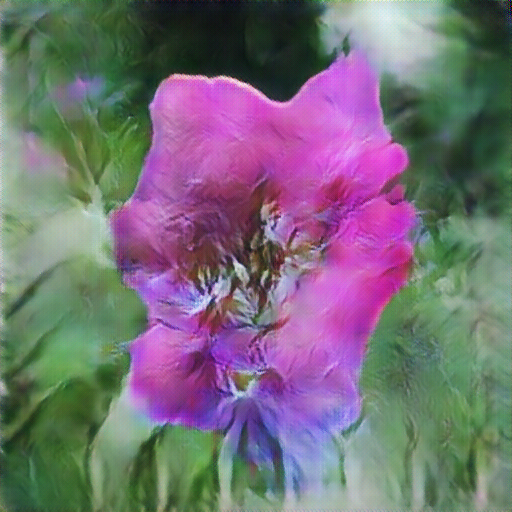
\includegraphics[width=.47\textwidth]{images/fixed_125_1}
        }
        \subcaptionbox{\label{sfig:rnd_125}}{
            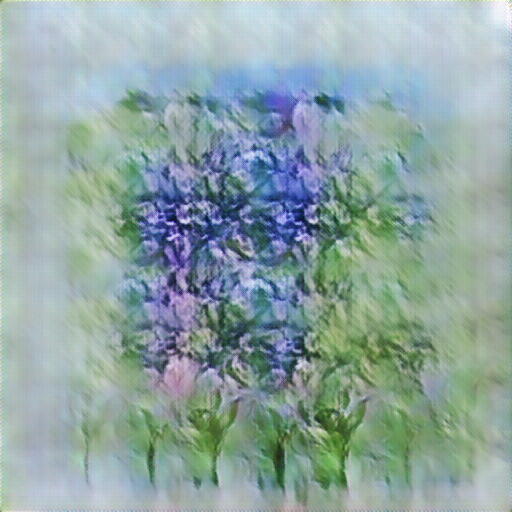
\includegraphics[width=.47\textwidth]{images/randomstatic_125}
        }
        \caption[Image generation with differently distributed latent code]
        {
            \textbf{Image generation with differently distributed latent code. The generator was trained on the distribution from the FMA dataset~\cite{FMA}. Latent code from the proper distribution~\subref{sfig:fixed_125} and from a multivariate normal distribution~\subref{sfig:rnd_125}.}
        }
        \label{fig:distribution}
    \end{figure}
    
    \section{DCGAN}

        Instead of pooling layers DCGAN uses convolutional layers in the discriminator to reduce the image resolution and transposed convolutional layers in the generator to increase the image resolution, an example can be seen in Figure~\ref{fig:architecture_dcgan}.
        
        \begin{figure}[h]
            \centering
            \fbox{
                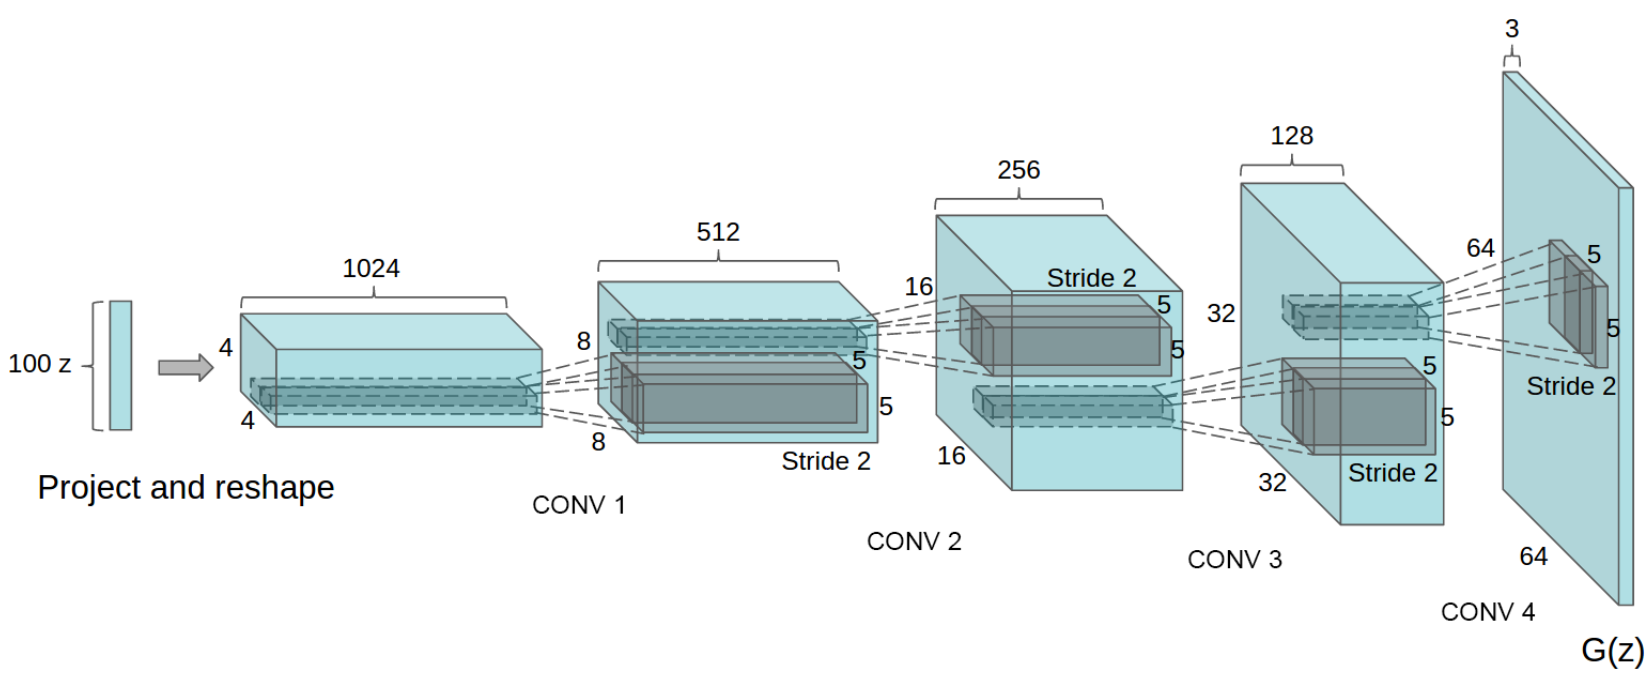
\includegraphics[width=.94\textwidth]{images/architecture_dcgan}
            }
            \caption[DCGAN generator for LSUN]
            {
                \textbf{DCGAN generator used for LSUN scene modeling. A 100 dimensional uniform distribution \vec{Z} is projected to a small spatial extent convolutional representation with many feature maps. A series of four fractionally-strided convolutions (in some recent papers, these are wrongly called deconvolutions) then convert this high level representation into a 64 × 64 pixel image. Notably, no fully connected or pooling layers are used.\\
                \textit{Figure and caption from} \citetitle{dcgan}~\cite{dcgan}.}
            }
            \label{fig:architecture_dcgan}
        \end{figure}

        Our first implementation was based on an implementation for CIFAR10. Because we want images with a resolution of more than 32 x 32, we scaled up the networks to fit our requirements.

        \subsection{Generator}

            As the input resolution for the generator is essentially 1 x 1, the first transposed convolutional layer of the generator, with a kernel size of 4, a stride of 1, and a padding of 0, outputs a resolution of 4 x 4. With an exception of the last, the remaining transposed convolutional layers double the resolution by instead using a stride of 2 and padding of 1 with the same kernel size. The last one uses a kernel size and stride of 1 and padding of 0, it is simply used ot reduce the channels for the final image, in our case 3.
            
            To reach our desired resolution of 512 x 512, we opted to increase the amount of layers rather than modify the stride and kernel size. This lead to an increase of transposed convolutional layers from 5 to 9. With the first and last having their own role, this leads to 7 layers doubling the resolution of 4 x 4 ($\rightarrow 4 \times 2^7 = 512$). While the original version reduced the amount of channels by a factor of two after each transposed convolutional layer, due to hardware limitations this method was no longer feasible after increasing the amount of layers. Instead we therefore reduced the amount of channels in the generator linearly. Due to a mistake during the first implementation and to keep backwards compatability, the last layer in the generator is scaled with 2$\times$ngf instead of 2$\times$ngf, with ngf being a variable that controls the size of the network. Each layers amount of output channels decreases in a linear fashion, with layer 8 having 2$\times$ngf filters, layer 7 has 4$\times$ngf, layer 6 has 6$\times$ngf, .., and layer 1 has 16$\times$ngf. The final architecture of our generator is displayed in figure~\ref{fig:architecture_dcgan_ours_generator}
        
            \begin{figure}[h]
                \centering
                \fbox{
                    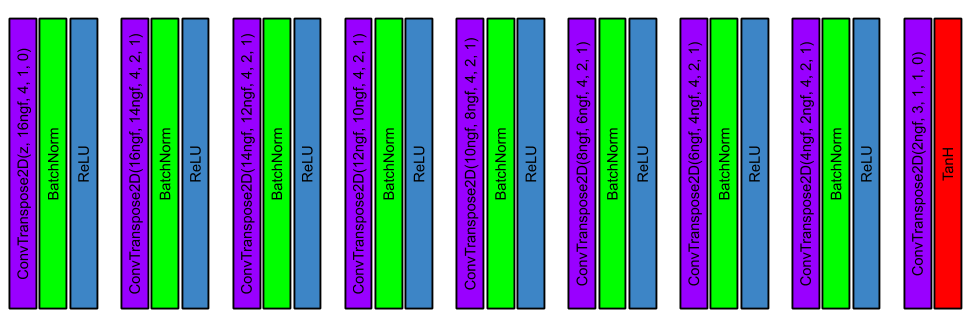
\includegraphics[width=.94\textwidth]{images/architecture_dcgan_ours_generator}
                }
                \caption[DCGAN generator architecture]
                {
                    \textbf{Architecture of our DCGAN generator that can be scaled with ngf and has a variable size of the latent vector \vec{z}.}
                }
                \label{fig:architecture_dcgan_ours_generator}
            \end{figure}

        \subsection{Discriminator}

            For the discriminator we applied the same approach. While the generator network increases the resolution while decreasing the amount of channels, the discriminator reduces the resolution and increases the amount of channels. The first convolutional layer starts out with the 3 input channels of an image, which are then increased linearly as we progress through the network. The exact architecture can be seen in figure~\ref{fig:architecture_dcgan_ours_discriminator}. Since the smallest transposed convolutional layer in the generator has 2$\times$ngf filters while the discriminators smallest convolutional layer has $\times$ndf filters, the generators network is more complex by default when ngf=ndf.

            \begin{figure}[h]
                \centering
                \fbox{
                    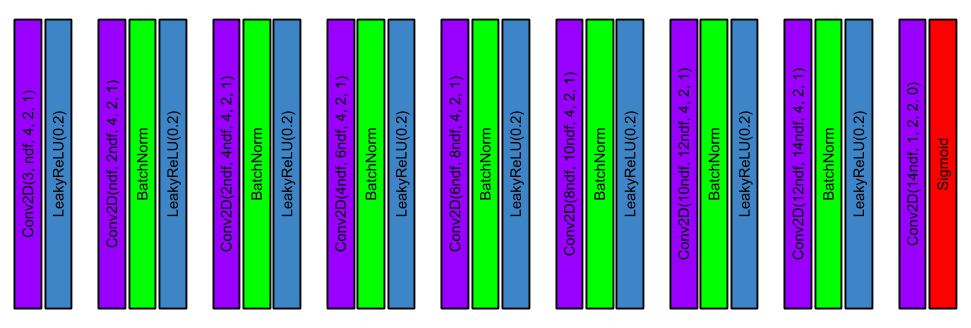
\includegraphics[width=.94\textwidth]{images/architecture_dcgan_ours_discriminator}
                }
                \caption[DCGAN discriminator architecture]
                {
                    \textbf{Architecture of our DCGAN discriminator that can be scaled with ndf.}
                }
                \label{fig:architecture_dcgan_ours_discriminator}
            \end{figure}

        \subsection{Training}
            We have found that training with values for ngf between 64 and 128 generate images of comparable quality.

            \TODO{
                training with actually possible input configurations allows for a more reasonable mapping of the feature space to output images. as an example, include an image of how 4 different input vectors result in almost the same output img when gan is trained on random input! more blah. Use example images for some epochs, displaying how the network improves over epochs. Important: explain that sample images not necessarily correlate to good video results! because of that we implemented static image sampling for important sections in songs (e.g. there's always a base-image for when almost nothing happens in a song! that one is important to look at when selecting a GAN state)
            }

            \begin{itemize}
                \item how are both networks trained?
                \item loss, optimizer, ..
                \item we changed the sample generation during training to contain some static useful vectors
            \end{itemize}

    \section{InfoGAN}

        Idea is to now use a conditional GAN to introduce some random noise into the image generation while ensuring the latent code has a high impact on the image generation. Using random input together with the latent code may cause abrupt changes between subsequent images.
        \begin{itemize}
            \item image of architecture
            \item mention loss, optimizer, ..
        \end{itemize}